\documentclass[12pt]{article}
\title{Report iteration 3 - SWOP}
\author{Dieter Geboers, Wouter Schaekers, Stefaan Truijen\\ - \\ Professor: Tom Holvoet \\ Project Advisor: Marko van Dooren}
\date{2012-04-06}
\usepackage[pdftex]{graphicx} % fotootjes
\usepackage{fancyhdr} % coole template
\usepackage[top=20mm,bottom=20mm,left=20mm,right=20mm]{geometry} % size and margins
\usepackage{hyperref} % for urls
\usepackage{listings} % code style
\pagestyle{fancy} % ook coole template
\begin{document}
\maketitle

\section{Preface}
This iteration is the final one. The new assignment instructed us to update our project so that it is able to support multiple campuses on hospitals. With this new feature came a new feature for doctors as well. Doctors gained the ability to travel between campuses. They also get a say in their behaviour concerning travelling between campuses: go back and forth between all campuses, or rather have an own schedule concerning locations? \\
\newline Preemptive scheduling and tasks that support multiple priority levels were not part of our assignment as we're a team of three members. \\
\newline We delivered a report on the refactoring changes we planned to execute during this iteration as well as two test scenarios for our system. However, as we changed the way the system works, the test scenarios were forced to be adapted. We also thought that it would be best to create an additional testing scenario to prove that the "basics" are not the only thing we can do. \\
\newline Our project advisor, Willem Penninckx, was replaced by Marko van Dooren for this iteration due to illness. We had some very constructive meetings with them both and are very thankful for the insight they gave us. Especially when we started to deviate from the core of the  project by over thinking some of the design decisions.\\
\newline For the first time in our SWOP history we can say with confidence that everything works like it should and there are no missing features.

\pagebreak
\tableofcontents
\pagebreak

\section{Introduction}
During the feedback session of iteration two, some major (asw ell as minor) issues with our code and design floated to the surface:
\begin{itemize}
\item{MachinePool had hard coded methods to create different types machines;}
\item{There were no system sequence diagrams available;}
\item{The UML of the domain layer did not have any relevant methods on it;}
\item{The implementation of Warehouse was lacking in a lot of aspects: }

\item{When an activity that required something from a warehouse got scheduled, there were no items removed from that warehouse;}
\item{The way Warehouse kept track of it's items and their maximum capacity was hardcoded;}
\item{The system for creating stock orders and delivering them to the warehouse wasn't implemented successfully;}
\item{\dots}
\item{The unit for time (milliseconds) used in the system was nowhere documented.}
\item{Some methods and controllers required the same set of parameters and instead of an object that groups them together, they were all mentioned explicitly.}
\item{...}
\end{itemize}
We have taken all of the above (and more) into account while implementing iteration three to make certain that our hard work would not have been in vain.
In this report we'll motivate the necessity of changes we have put the project through. Also, we'll try to give some other solutions for the problems we encountered that caused us to create the system as it is. We'll then draw a conclusion and leave it at that. \\
\newline As for the amount of time we spent working on this iteration in detail, we refer to \url{http://code.google.com/p/swop-dswx/wiki/WorkingHours} . We have worked on this iteration for about 150 hours. Implementing accounts for a rather small percentage of this number. Most of the time we found ourselves thinking and discussing design decisions.

\section{Package visible constructors}
We decided to make as many constructors as we could package visible only. Doing this denies the creation of the affected objects by any unwanted classes/people efficiently. However, the lack of friend classes and friend packages in Java made it impossible to protect every constructor of every class in such a way. \\
If such a class or method exists, there will be documentation stating that the method or class in question should never be used outside of the domain layer.\\
For example: once Machine objects get created, they are added to a MachinePool immediately. The responsibility of assigning every Machine to a MachinePool lays with the MachinePool itself.

\section{Creational design patterns}
The following problem presented itself to us a couple of times while developing a plausible design for the assignment: what is a \emph{clean} way to allow users to create new objects of certain dynamically changing classes? For example: how can we make sure that the user  has the ability to create a new ultra sound scanner without making the domain inconsistent or giving too much responsibility to the user interface?\\
An answer to this question is implementing a creational design pattern. We decided to use a builder pattern for the creation of new Machines and an abstract factory pattern for the creation of new Users, Treatments, MedicalTests.\\
The builder mentioned above is nothing like the StandardHospitalBuilder, ExtendedHospitalBuilder, WarehouseBuilder, UserManagerBuilder,... that you may have noticed in the source code of our project. In fact, they're nothing alike. The latter builders are templates for an initialised system to avoid a bunch of code duplication across different testing units.\\
\newline Without further a due, we will now briefly discuss the creational patterns mentioned in the paragraph above.

\subsection{User factories and user manager}

\begin{figure}[h!]
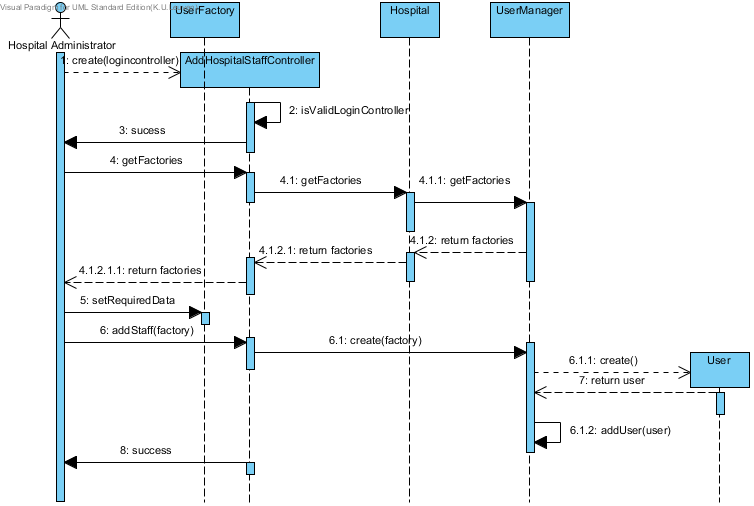
\includegraphics[width=175mm]{addstaff.png}
\caption{The sequence diagram from the add hospital use case demonstrates how user factories are to be used and how they work in the domain layer.}
\label{addHospitalStaffSD}
\end{figure}

First, let's take a look at the sequence diagram of add new hospital staff above. We can see that the hospital administrator asks a list of all available factories, then selects the kind of factory he would like to create a new staff member from, next sets the required parameters and then lets the system create such a user.\\
The creation of the actual User object is the responsibility of the UserManager. This makes it easy to make certain that, when the user uses the public controller API, it's impossible to create a new User object that's not kept in a UserManager.

\subsection{Machine builder and machine pool}
Blood analysers, x-ray scanners and ultra sound scanners all have the same signature in their constructors. They also do not have any specific characteristics other than their types. This is the reason we chose to use a builder design pattern as a solution to the creational problem described in the beginning of this chapter.\\
It is also important to note that the constructor and build()-method of each builder is package visible only. This means no new MachineBuilder objects can be created without going through the MachinePool. Also the constructors of each of the machine types are package visible only. The combination of these visibility limitations means that, analogous to the case with UserFactory and UserManager, creating a new Machine or MachineBuilder object without registering it in a MachinePool is impossible.\\
Alas, the visibility in Java is not what it could be. We were forced to make the Machine classes themselves public as we require Machine objects in other packages. In particular, packages that contain TaskDescriptions come to mind, but more on that later.

\begin{figure}[h!]
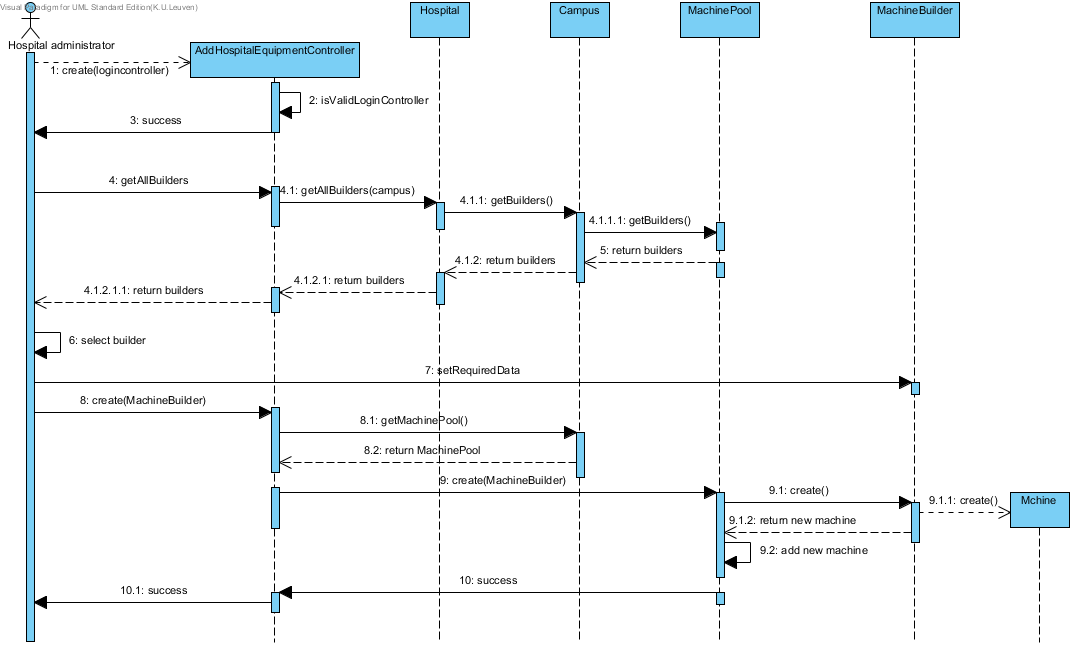
\includegraphics[width=170mm]{addequip.png}
\caption{A sequence diagram of the add equipment use case}
\label{addequipment}
\end{figure}

\subsection{Medical test factories and patient files}
When a doctor wants to order a new medical test for a patient, he or she will create a new OrderMedicalTestController. This controller allows the doctor in question to get all existing medical test factories. These factories are stored in the Hospital class and should be added manually at initialisation time before any use cases can be executed.\\
Once said factories have been acquired from the controller, the doctor can specify the required details in order for the medical test he's about to order to be exactly as he or she would like it to be. The doctor then calls upon the controller one more time, giving it the pre-set MedicalTestFactory. The controller passes this factory on to the task manager. The task manager executes the create()-method. This method generates a new MedicalTestDescription. This description is then stored in a new Task. The Task is then initialised (which means it will be stored in the patient file of the patient who the medical test is for).\\
We would have preferred for the create()-method to have limited visibility. Once again Java does not provide us with the possibilities to do so. Therefore we have equipped it with the \texttt{@Deprecated}-annotation so that, should someone try to call this method, they will see that it's not meant to be called. The documentation of the create()-method also informs the reader of this.\\
Like before, this way of things allows for a reliable domain layer to be constructed and maintained throughout the execution of the program. No MedicalTest objects will ever exist without there being a Task, as well as a PatientFile, to store them. The way Tasks are created (by first creating descriptions and then transforming them into Tasks in the TaskManager) also assures that Tasks never exist created without a TaskManager keeping track of them. Also, we would like to note that the constructor of Task is package visible within the scheduler.tasks package to aid in achieving this goal.
\subsection{Treatment factories and diagnosis}
Treatment factories allow doctors to create treatments that are always linked to diagnose similar to the way medical test factories allow doctors to create medical tests that are always linked to a patient file.\\
The doctor creates the appropriate controllers and asks them for the treatment factories available in this hospital. Just like is the case with medical test factories, these treatment factories are to be initialised at system initialisation time before any use cases can be ran.\\
The doctor chooses one of the given treatment factories and sets the required data. Then the doctor gives the factory back to the PrescribeTreatmentController, who then in turn, gives it to TaskManager. The TaskManager then creates a description from the factory and transforms it to a Task. The created Task gets initialised, which causes it to be linked to the diagnose it was created for.
\subsection{Diagnosis and patient files}
No Diagnose objects should exist without there being a PatientFile object to store them. The sequence diagram below demonstrates how assuring this consistency happens when the controllers are used properly:

\begin{figure}[h!]
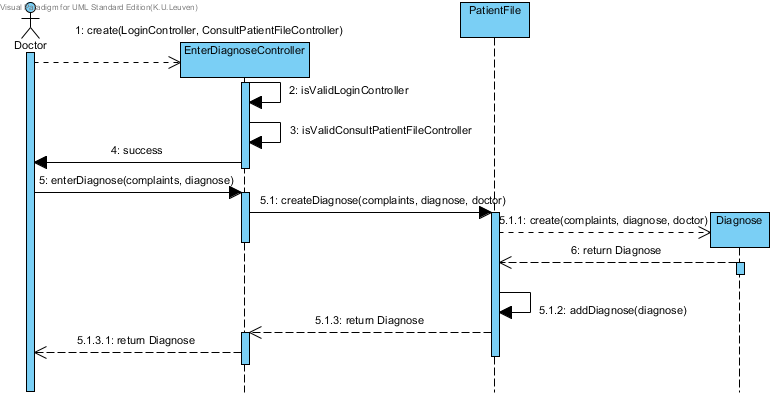
\includegraphics[width=170mm]{enterdiagnose.png}
\caption{The sequence diagram of the enter diagnose use case demonstrates how no diagnose can be created without a patient file storing it.}
\label{enterdiagnose}
\end{figure}
\subsection{Warehouse builder and campus}
Warehouses should not exist without a StockProvider (see later). Also a campus should always have a warehouse. To make this possible we use WarehouseBuilder objects at initialisation time. These warehouse builders are not design pattern builders but merely a way to assure the desired consistency mentioned above at creation time.

\section{Task}
Task object represent task concepts from the real world. Tasks are created from descriptions and are stored in the TaskManager. Tasks can undergo 2 transformations in their lifetimes. When they are created, they are regarded to as queued tasks. When the opportunity presents itself, the queued task becomes a scheduled task. Once the scheduled task has been executed, it becomes a finished task.
\subsection{Generic tasks versus a hierarchy of tasks}
Tasks come in many different forms. In the last iteration, we worked with a hierarchy of Task objects. For example: UnscheduledMedicalTestTask, ScheduledMedicalTestTask, UnscheduledTreatmentTask, ScheduledTreatmentTask, \dots . During a meeting with our project advisor, we came to the conclusion that such a hierarchy is not very desirable and violates the GRASP patterns. We then chose to work with a generic Task class: \texttt{Task<? extends TaskDescription>}. "Tasks from task descriptions".\\
The class diagram from Tasks and their descriptions can be found in figure ~\ref{taskuml} .

\begin{figure}[h!]
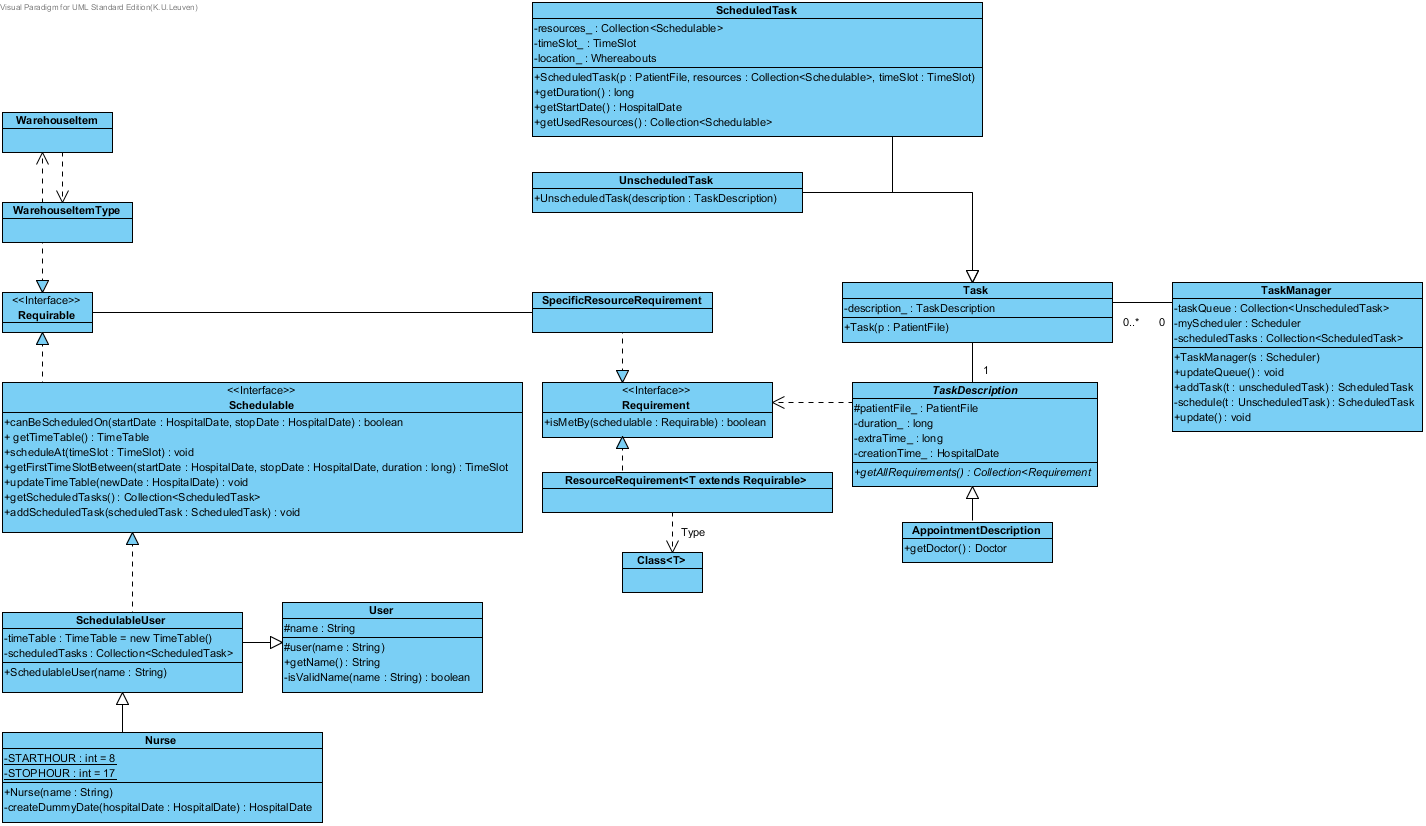
\includegraphics[width=220mm,height=160mm,angle=90]{Task-Description.png}
\caption{Tasks and their descriptions}
\label{taskuml}
\end{figure}

\subsection{The state of a Task}
As described in the beginning of this chapter, tasks undergo "transformations". These transformations are implemented with a state pattern.\\
A task keeps its TaskState. The existing TaskState objects are: QueuedState, ScheduledState, FinishedState. Each state keeps a TaskData object. This object stores information relevant to the current state of the task. For example: a queued task would only keep its description while a scheduled task also keeps all resources involved in the execution of the task, where the task is to take place, etc\dots
\subsection{The description of a Task}
We define tasks by their description. Examples of these descriptions are: blood analysis, surgery, medication, appointment,\dots \\
These descriptions can be created using the controllers and the factories they can provide the user with. Once created, a description gets stored in the task data of a new queued task. A description contains requirements and conditions  specific for that description. These requirements and conditions need to be met in order to schedule the queued task. (see later) You can find a diagram of these states below in figure ~\ref{taskstate} .

\begin{figure}
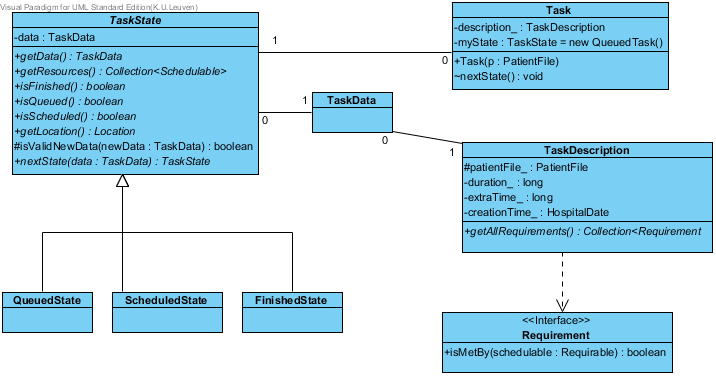
\includegraphics[width=150mm]{TaskState.png}
\caption{Tasks and their states}
\label{taskstate}
\end{figure}

\section{Warehouse}
During this iteration we also made some large refactoring, if not implementing from scratch, from everything related to warehouses. There were a couple of significant problems, like mentioned in the introduction of this report. We managed to successfully find clean solutions for them all.\\
Let's take a look at the class diagram from warehouse first: 

\begin{figure}[h!]
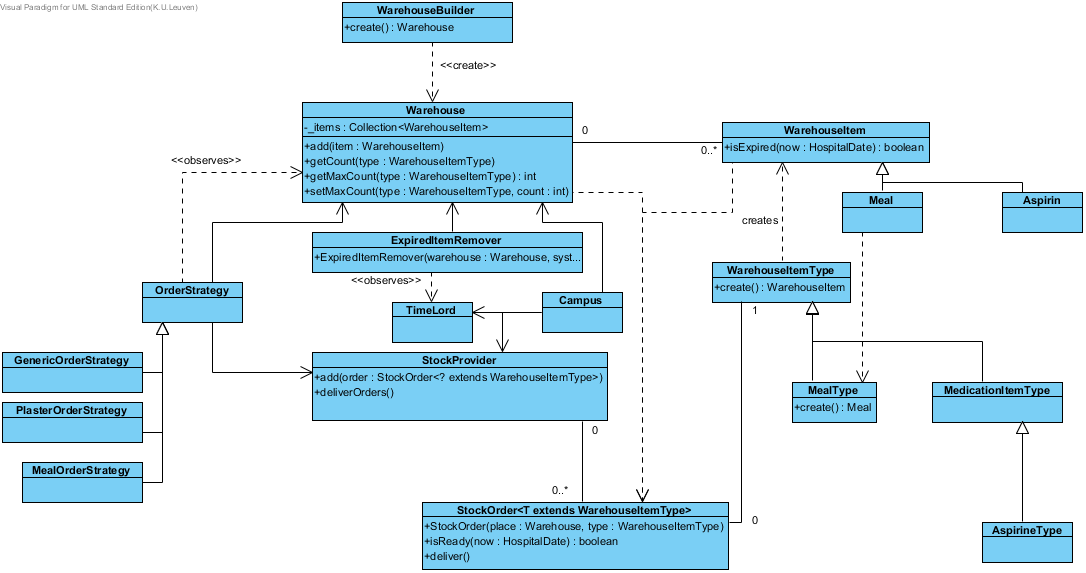
\includegraphics[width=170mm]{Warehouse.png}
\caption{Class diagram from warehouse and its related classes}
\label{warehouse}
\end{figure}

The basic idea is that, using a WarehouseBuilder, we connect an ExpiredItemRemover and as many OrderStrategies to the warehouse as needed.\\ OrderStrategy is a class that, when the item type it's observing is running low, creates new stock orders for the warehouse automatically.\\
As different types require different methods of 
ExpiredItemRemover observes the current system time. Should the time change, the item remover will check if there are items in the warehouse that have expired due to the new system time and will remove them. This removal will, evidently, trigger order strategies to be notified.\\
All newly created stock orders are kept in the stock provider. The stock provider also observes the current system time. When the time changes, the stock provider will attempt to deliver all deliverable stock orders. Stock orders are deliverable if the required time to pass between order creation and the new system time is sufficient.\\
The stock provider is created together with the warehouse and both are stored in the campus. Working with only one stock provider per campus makes it easy to create the exact amount of new stock orders required.\\
The warehouse stores 

\section{Scheduling}
The Scheduling algorithm is built in such a way so that the Scheduler doesn't know anything about the specific classes that are in the the rest of the domain layer. It only knows about abstract schedulables and requirements.
\subsection{Description and Requirements}
A Description is an abstract class that \textit{describes} a possible task. Such a Description can be an Appointment, a BloodTest, \dots.  It has all the information it needs to be able to build a task. This information is contained in the form of requirements. A Requirement is a class such as a Doctor, a WarehouseType, a Nurse, \dots. Requirements know what Objects are needed to forfill this Requirement. There are different Requirements, since not all Requirements are not of the same type:
\begin{itemize}
\item SpecificRequirement: This kind of Requirement contains one Object that needs to be fulfilled. For example a Doctor during an Appointment. This Requirement will only be met by this Doctor.
\item RequirementType: This kind of Requirement contains an ObjectType. All Objects of this type will fulfill this Requirement. It is possible that there are more than one Object needed to fulfill this Requirement. This information is also stored in this Requirement. An example of this kind of Requirement are Nurses during a xray scan. Since it is not important which Nurse does the scan, only some Nurse object is enough to fulfill this Requirement.
\item DiagnoseCondition: This kind of Requirement is only fulfilled if the diagnose of the patient is approved.
\item WarehouseItemCondition: This kind of Requirement can only be fulfilled if a Warehouse has enough items of the kind of type that is stored in this condition. To check whether this condition is met, a HospitalDate and a Location is needed to check this Condition. This Requirement has a collect method, in order to delete all the items it needs from the given Warehouse.
\end{itemize}
All these Requirements have the same interface, and thus the same methods. One of the methods is \textit{isCrucial()}. A Requirement is crucial if the Requirement needs a Machine or a SchedulableUser. This Requirement can only be met when the admin adds Machines or SchedulableUsers to the Hospital. If this Requirement is not met, the Task can never be scheduled in this Hospital with the current resources. If there are not enough resources available in the hospital to forfill this Requirement, the Task will never be able to be Scheduled and will be deleted from the system.
\subsection{Scheduler and TaskManager}
Due to security reasons, it is impossible to create Tasks. A user can only make Descriptions. If a Description is made, the user is obliged to add this Description to the TaskManager. The TaskManager will make a Task out of it and tries to schedule it immediately after that. The scheduling happens with a scheduling algorithm in the Scheduler class. It will try to schedule this task. It is possible that the Scheduler is not able to schedule the Task. In that case, the Scheduler will throw an exception. There are two types of exceptions. Depending on the sort of the exception, the TaskManager will decide whether it will store this Task in a queue or will throw it away.\\
During this process, the description will be initialised. During this initialisation, the DiagnoseCondition will start observing the Diagnose, in case the state of the Diagnose would ever change. The TaskManager will aslo has to observe the Task, so the Diagnose will notify the TaskManager indirectly.\\
If the Scheduler is able to schedule the Task, it will schedule all Schedulables and collect all the WarehouseItems. The state of the Task will be changed.
\subsection{Schedulable and Requirable}
Schedulables are Objects that can be scheduled. They have a TimeTable.\\*
Requirables are Objects that are needed to forfill a Requirement. This is in fact just an empty interface to generalize all the Objects that are usefull for this.

\subsection{HospitalDate}
We had started implementing the system that’s in the class diagram above by using java.util.Date. We soon found out that there was something not right with this library. The methods used to get the year, date, hour,… of a Date-object are all depricated and do not work at all in combination with the not-depricated constructor and toString() of Date. After numerous frustrations about Date, we considered a number of possible alternatives.
\\The most evident alternative would be java.sql.Date. However, this library does not vary all that much from java.util.Date and we found it just almost just as dysfunctional as the latter. The next possible solution was to work with Calendar objects from java.util.Calendar. Unfortunately using this class is not as programmer friendly as one would expect it to be. We would like to quote Joshua Bloch, Google's chief Java architect and author of “Effective Java”, from an interview in which he was asked to give some tips for Java developers. In this interview, he said the following:
\begin{center}
\emph{"As an extreme example of what not to do, consider the case of java.util.Calendar. Very few people understand its state-space -- I certainly don't -- and it's been a constant source of bugs for years." - \url{http://java.sun.com/developer/technicalArticles/Interviews/bloch_effective_08_qa.html} .}
\end{center}
We then opted to go with java.util.GregorianCalendar instead. While a significant improvement over Calendar, GregorianCalendar still proved to be rather hard to work with. Finally we decided to write our own Date class and named it HospitalDate. This class uses the GregorianCalendar to store and calculate dates, but we implemented some getters and setters so that using a HospitalDate would make our code easier to read and write. HospitalDate turned out to be exactly what we needed as it did not have any of the disadvantages of the other alternatives mentioned above.
\newline HospitalDates have a constructor that allows you to create a Date that takes place at a certain amount of milliseconds since the system start time (8AM at Nov 8th, 2011): the so called "start of time". "End of time" is the point at which the value of long would overflow, if added one more millisecond. All methods returning milliseconds or asking milliseconds as a parameter work in this way. 

\subsection{TimeTable}
A TimeTable is a class that represents the individual TimeTable that each Schedulable has. It very much resembles a real life timetable in which one can keep track of one’s appointments and todos. A TimeTable consists of a set of TimeSlots. Each TimeSlot in the TimeTable represents an interval in time during which the TimeTable in question is marked as being “occupied”. A couple of methods in TimeTable that are worth mentioning (as they're not in the class diagram):
\begin{itemize}
\item{invert() : TimeTable}
\item{getUnion(TimeTable) : TimeTable}
\item{getIntersect(TimeTable) : TimeTable}
\item{eliminateOverlap() : void}
\end{itemize}
Invert() inverts the TimeTable. This means: busy slots become free slots and the other way around. The result of this method is a new TimeTable that is the inverted one of this TimeTable. Evidently the inverted TimeTable of the inverted TimeTable of an original TimeTable, is the original TimeTable again. This method can be very useful to determine all free slots in a  TimeTable. 
\\*getUnion() gets the union of two TimeTables. The union is defined analogous to the union of two collections in mathematics: it’s a new TimeTable that is marked as “busy” everywhere where either one or both of the original TimeTables is “busy”.
\\*getIntersect() gets the intersection of two TimeTables. Like getUnion(), getIntersect() is defined very much like in mathematics: the intersection of two TimeTables is a new TimeTable that is marked as “busy” where both of the original TimeTables are “busy”.
\\*eliminateOverlap() is a method that basically merges timeslots that overlap. For example: if a TimeTable contains a slot from 5AM to 8AM and another one from 7AM to 9AM, eliminateOverlap() will result the two original timeslots being reduced to only one: from 5AM to 9AM.

\subsection{TimeSlot}
A TimeSlot is nothing more than a representation of an interval of time. It has a starting- and stopping point. Its length is in milliseconds.

\subsection{TimePoint}
As a TimeSlot has a starting and stopping point, TimePoint is the abstract class that represents those points in time. Each TimePoint has a HospitalDate so as to know which point in time it really represents.
\\*It has two child classes: StartTimePoint and StopTimePoint. At first TimePoint held on to an enumeration so that it would know whether it was a starting- or stopping point. Now however, the design is more adaptable: it's easily possible to add a new sort of TimePoint now due to the high cohesion achieved by using two separate classes.

\subsection{Schedulable and SchedulableUser}
Schedulable is an interface that is implemented by all objects that can be scheduled in the hospital (i.e.: nurses, doctors, XRay scanners, bloodanalysismachines,…). Because hospital administrators and warehouse administrators can’t be scheduled for now, there is also a distinction between User and SchedulableUser, as you can see in the class diagram.
Schedulable objects have three methods worth mentioning: 
\begin{itemize}
\item{canBeScheduledOn(HospitalDate startDate, HospitalDate stopDate) : boolean}
\item{getTimeTable() : TimeTable}
\item{scheduleAt(TimeSlot timeslot): void}
\end{itemize}
These methods should do what their names suggest they do. canBeScheduledOn() will return true if the object executing the method finds that all it’s privately kept constraints have been met and that its TimeTable allows it to be scheduled at the given interval of time. getTimeTable() will get and return the TimeTable of the Schedulable in question. scheduleAt() will schedule the Schedulable at the given TimeSlot if possible.

\subsection{Constraints}
There are a lot of constraints related to time and scheduling in this assignment. I.e.: nurses only work between 8AM and 5PM, Treatments can be registered before being scheduled, everything must be scheduled at least 1 hour in advance of the current system time, a patient may only get ten XRay scans per year,\dots. Most of these constraints can be taken care of by canBeScheduled() in Schedulable. 
\\*A constraint that has risen a problem was the fact that a Diagnose can already have a Treatment without it being scheduled if the Diagnose is not approved yet at the time of the creation of the Treatment. We'll elaborate on this in the sections below.

\subsection{Task, UnscheduledTask, ScheduledTask, TaskManager}
Task, UnscheduledTask and ScheduledTask are all abstract classes that represent things that can be (or already have been) scheduled. UnscheduledTasks are Tasks that haven't been scheduled yet. Once they can be successfully scheduled by Scheduler, they can be removed from the task queue kept by TaskManager and turned into ScheduledTasks. The ScheduledTasks get stored in the Schedulables that are to execute the ScheduledTask so that giving the user sensible output concerning todos is almost trivial.
\\* As is, it is possible a Task can't be immediately scheduled after creation. Possible reasons for this could be: the warehouse has run out of stock of an item required by the Task that was just created or the Task that can't be scheduled is a Treatment for a Diagnose that has not been approved yet. We managed to solve both of those problems by implementing the observer pattern. We now have a couple of Observers that get notified at the right times and that then tell the TaskManager to update its queue as some changes in the system has triggered the observer watching it.

\subsection{TimeLord}
TimeLord is the class that keeps track of the current system time. We have chosen to create a seperate class for that purpose only. The alternative was to keep the current system time stored in Scheduler. However, we felt like this does not fall under the responsibilities of Scheduler. 
\\*Let's assume one would like to keep the current system time in Scheduler. They then would have to make a choice between having the system time be static or not. A static system time is bad for the following reason: any class extending scheduler will not be able to keep their own system time should another scheduler or sub class of Scheduler already exists. Expanding the hospital into several timezones or creating a new sort of Scheduler, would then not be possible. The only option left then is to keep it as a non-static field. That would mean that any class requiring the system time would depend on Scheduler. This is bad for low coupling and high cohesion as a very high amount of classes will then depend on the Scheduler.

\subsection{Impact of having different locations}
The different locations had a huge impact on the scheduling algorithm. Instead of just iteration over all the resources, the algorithm had to take into account that not all resources are available everywhere. This has been eleganlty solved, by just iterating over all the locations and then trying to schedule over there. The scheduler will chose the best timeslot amongst all the possiblities.
\subsection{The location preference for doctors}
Because different campusses were introduced, doctors had the option to switch between them. In order to solve this problem, we introduced states. There are two different states. A selected preference state and a back and forth state. The purose of these two states is handling the TimeTable-calls. This is possible since every state has a LocationTimeTable. All the calls on Doctor involving the gathering of TimeSlots will be overriden and redirected to the states.
\subsubsection{getLocationAt()-method}
Since every state contains all the information about the location of the Doctor, the state is able to know where the Doctor is at every point in time.\\*
Because we were a little short in time, we didn't have the time to implement these methods.

\section{The updated testing scenario}
We have changed the testing scenario we handed in on the deadline of the refactoring report drastically. We will now give a short look into the setting of the new scenario and what it does.
\subsection{The state of the hospital at initialisation}
The hospital has one hospital administrator and two campuses.\\
Campus 1 contains: 
\begin{itemize}
\item{Three nurses: Jenny, Jenna, Jeffrey;}
\item{Four doctors: Jonathan, Jens, Jelle, Joanne;}
\item{Three x-ray scanners;}
\item{One ultra sound scanner;}
\item{one WarehouseAdministrator: Greg.}
\end{itemize}
Campus 2 contains:
\begin{itemize}
\item{Two nurses Joy, Janna}
\item{Two doctors Joe, Jennifer}
\item{Three blood analysers;}
\item{One WarehouseAdministrator: Geoff.}
\end{itemize}
The patient files and their history stored in the hospital:
\begin{itemize}
\item{Stefaan was diagnosed with "cancer" by Jonathan but the diagnose still needs a second opinion from Jennifer. Complaints are "sleepy". Patient has had a blood analysis in the past, created by Jonathan.}
\item{Dieter was diagnosed with "Hypochondria" by doctor Joanne. The diagnose has been approved. Patient's complaints are "Feel sick ALL the time".}
\item{Wouter was just registered in the hospital by nurse Jenna. Complaints are "arm hurts".}
\item{Thibault is currently discharged. Has had the following MedicalTests in the past: one UltraSoundScan, one XRayScan, one BloodAnalysis. Was diagnosed with "Fatal new variant of pneumonia" and had the following treatment carried out successfully: a surgery "Lung transplant".}
\end{itemize}
After this hospital state has been initialised, the test scenario gets executed.
\subsection{The events that occur}
\begin{itemize}
\item{Stefaan gets a new MedicalTest: BloodAnalysis. Jennifer disapproves the previous diagnose after the blood analysis has been carried out. The replacement diagnose is "stress". This diagnose gets reviewed and approved by Jonathan. The medication treatment, created by Jennifer, gets scheduled and results in nothing abnormal. Stefaan gets discharged by Jens.}
\item{Dieter gets a brain surgery treatment. This treatment is carried out without problems. After the result of the surgery has been entered, Jens discharges Dieter.}	
\item{Wouter gets an appointment with Joe. Joe creates a blood analysis and an x-ray scan for Wouter. After both tests have happened, Joe concludes that Wouter has a fractured arm. The diagnose is approved without needed a second opinion after which a cast gets scheduled. After the result is entered, Wouter gets discharged.}
\item{Thibault enters the hospital at campus 1and complains: "stomach hurts, jaundice". Nurse Jenna checks him in and creates an appointment with Joe. Joe creates an ultra sound scan and an x-ray scan. From these medical tests, Joe concludes that Thibault's "liver is failling". The treatment is another surgery: "liver transplant". After the treatment has been carried out and the result has been entered, Thibault gets discharged.}
\item{Five new patients come into campus 1 and all of them have the same symptoms "pain in chest and difficulty breathing". After they get their equal appointments, tests, diagnosis ("Heavy metal poisoning") and treatments, two out of five survive while three of them didn't make it.}
\item{Advance time is called a multitude of times in the execution of this scenario.}
\end{itemize}
\section{Things that can be done better}
\subsection{Diagnose state}
The lack of the state pattern in Diagnose gave us many problems, we were to late to discover this and thus were unable to implement the pattern here. We think the states UNAPPROVED,APPROVED,DISMISSED would be very helpful in Diagnose objects.
\subsection{Comments}
We have a lack of commenting on our code, partially due to time pressure and thanks to the many overhauls in our design. The times that when an exception is thrown it is documented thoroughly is rare even in the controllers.
\subsubsection{TimeTables \& Locations} We noticed that the timetables were very helpful when we were dealing with one campus, but when multiple campi were introduced to the domain they were not sufficient. An ideal sollution would probably be a LocationTimeTable that saves the location of a Requirable with the time or a task timetable that keeps track of which task is being executed at what time. This would mean that the interface of Requireable would change and that occupiedOn(HospitalDate):boolean would change to getTaskOn(HospitalDate):Task, all the required info could possibly be derived from that object.
\subsection{Factories \& consistency}
We have a lack of consistency in where the create() method of a factory can and should be used. 
\subsection{DoctorState}
The state pattern in Doctor is used but not yet in such a way that is sufficient, Doctors don't travel  between campi. This has high cohesion with the TimeTable location problem that we faced and did not fix.
\subsection{Results} 
We had little problems implementing the results for different task in the hospital, but because we introduced them (as seperate objects) too late in our system they barely had any testing.
\section{Eclemma and unit tests}
We reached a +- 80\%  code coverage of our domain. We did little border case testing but most of the functionality is implemented. The warehouse package together with the scheduler and task package has the most coverage, we spend a lot of time on testing the timetables since they weren't easy to implement and are one of the most important classes of our system.
\section{Capsules}
After we've reviewed the design completely, we made all domain layer packages friends with eachother. The public API consists of all the methods in the controller-package and the set-methods from the used factories.\\
The controller package is a friend package of the ui package. The ui package does not have any other friend packages than the controller package.

\section{Conclusion}
After a lot of hard work with a lot of ups and downs, we feel that we now finally have a system that's designed in a very acceptable way that covers all the bases. Throughout the project several issues concerning team work surfaced and resurfaced. The main one being communication. Explaining what seems evident on the inside your head to other people who don't see things the same way you do can sometimes lead to faulty interpretations or even frustrations.\\
Nevertheless we learned a lot about object oriented programming, team work, the limitations of Java, design patterns and refactoring.
\end{document}